\section{Visualization and Analytical Framework}

\subsection{Interactive 3D WebGL Visualization Suite}
Raw tensors and covariance matrices do not readily convey the tactical urgency of a conjunction event. To bridge the gap between our G-PINN engine and operational decision-making, we developed a massive, bespoke 3D visualization suite utilizing \texttt{Three.js}.

The visualization engine comprises several ascending tiers of complexity (\textit{NasaEyesUltimate}, \textit{NasaEyesSupreme}). The pipeline preemptively computes 800 state vectors across a temporal window. We perform a real-time affine mapping transformation ($x \rightarrow x$, $z \rightarrow y$, $y \rightarrow -z$) to ensure visual congruence with standard 3D game engines. The Python backend dumps the fully corrected, massive array of 3D positional coordinates as a JSON string directly into a dynamically generated HTML template containing embedded JavaScript.

\begin{figure}[H]
\centering
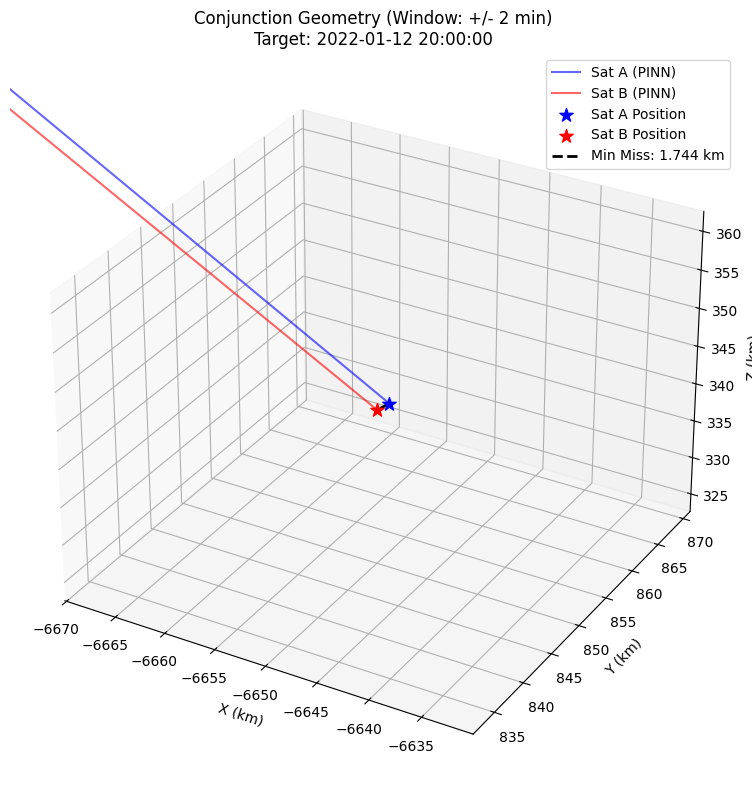
\includegraphics[width=\columnwidth]{figures/3D_Conjunction_Geometry.png}
\caption{3D conjunction geometry rendered in the WebGL decision-support interface.}
\label{fig:3d-conjunction}
\end{figure}

\subsection{Dynamic Follow-Camera Logic}
To accurately represent a conjunction that occurs at orbital velocities ($>7$ km/s), the engine employs a dynamic chase-cam lock:
\begin{equation}
    \text{Sat}_{B\_rel} = \text{Pos}_B - \text{Pos}_A
\end{equation}
The camera is anchored to the primary satellite at coordinates $(0,0,0)$. The entire universe---including the Earth model, the background starfield, and the intruder satellite---is dynamically shifted relative to Sat A.

\begin{figure}[H]
\centering
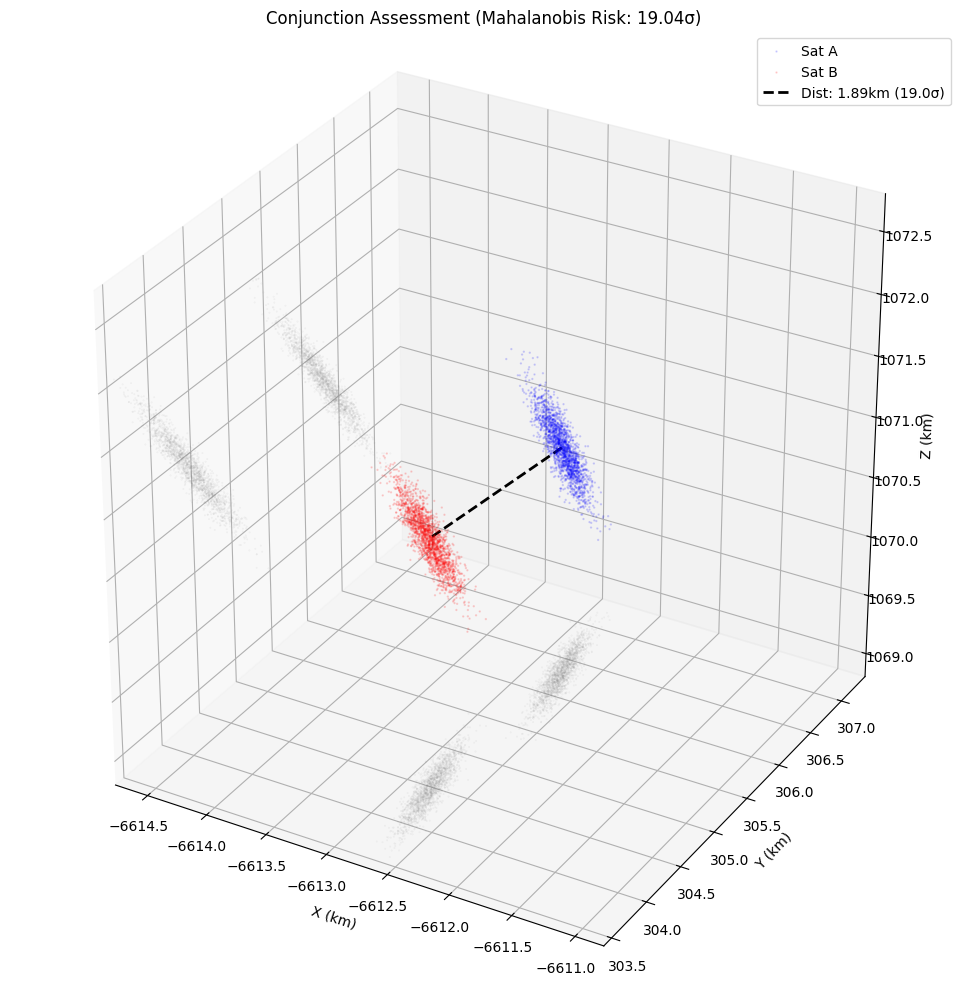
\includegraphics[width=\columnwidth]{figures/mahaanobis_risk.png}
\caption{Mahalanobis risk-density visualization for covariance-aware conjunction assessment.}
\label{fig:mahalanobis-risk}
\end{figure}

\subsection{Shadow Projections and Mahalanobis Confidence}
The visualizer projects 3D Monte Carlo covariance clouds into 2D shadows onto the $X, Y,$ and $Z$ limiting bounding planes. By rendering 10,000 parallel particle states colored by risk density, the visualizer provides an immediate heuristic of whether the primary asset's covariance ellipsoid intersects the intruder's, effectively communicating Mahalanobis risk.
